\documentclass[aspectratio=169]{beamer}

\title[Economic Feasibility of Residential Solar and Battery Colocation]
{Evaluating the Economic Feasibility of Residential Solar and Battery Colocation}

\subtitle{A Cost Optimization Approach}

\author{Xinyu Luo}

\institute{\footnotesize
Institute for Computing in Research
}

\date{July 30, 2026}

\begin{document}
\frame{\titlepage}
\begin{frame}
\frametitle{Background knowledge}

\begin{itemize}
    \item Why residential renewable energy, and why is it a popular option for homeowners?
    \item What is photovoltaic (PV) technology, and how does it work?
    \item What is residential PV-battery colocation?
\end{itemize}
\end{frame}

\begin{frame}
\frametitle{Benefits of colocation}
\begin{columns}

\column{0.6\textwidth}
\centering
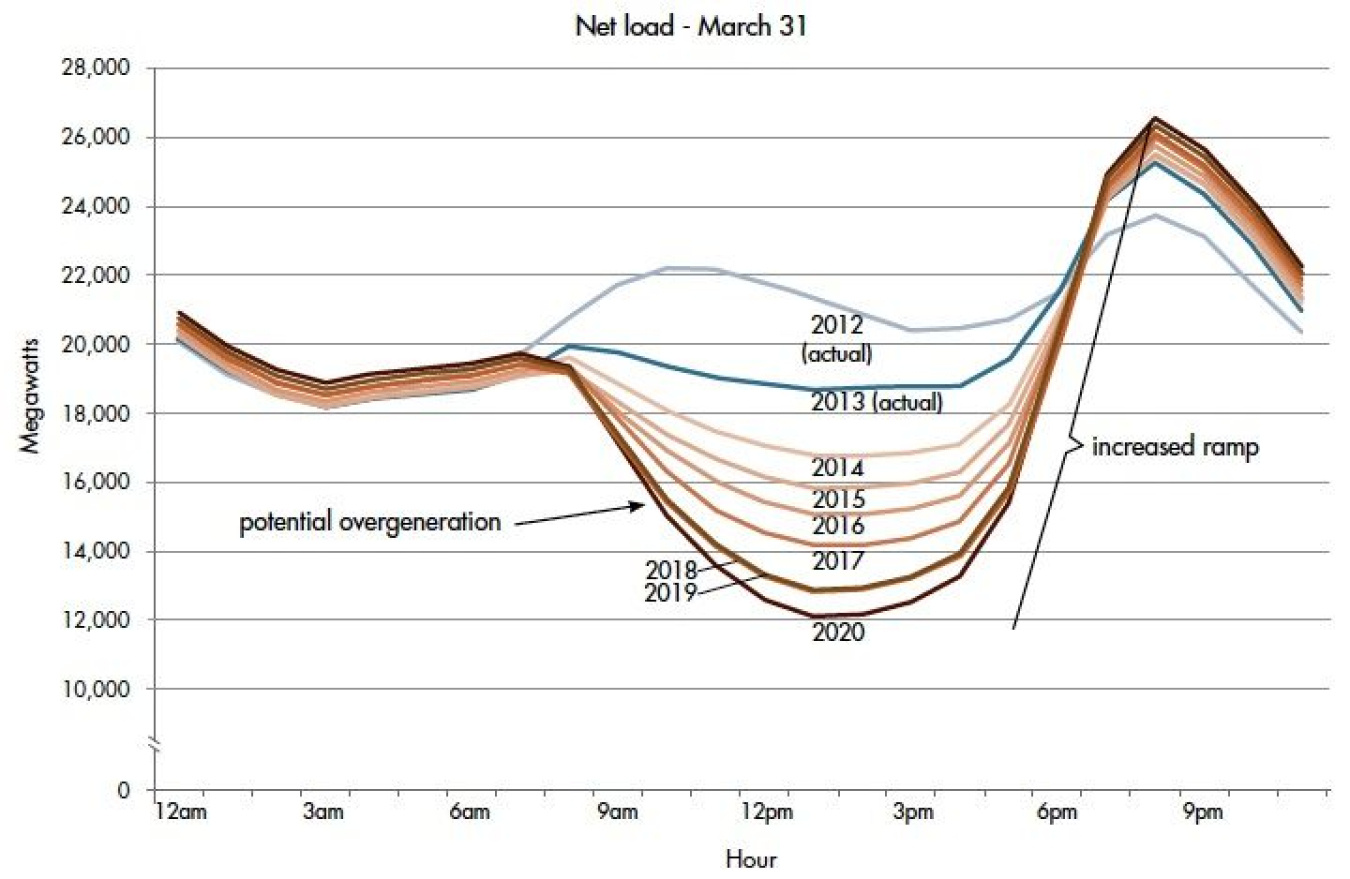
\includegraphics[width=\linewidth]{Duck-Curve.jpg}
\vspace{0.2cm}
\small Duck curve (Jones-Albertus, 2017).

\column{0.48\textwidth}
\centering
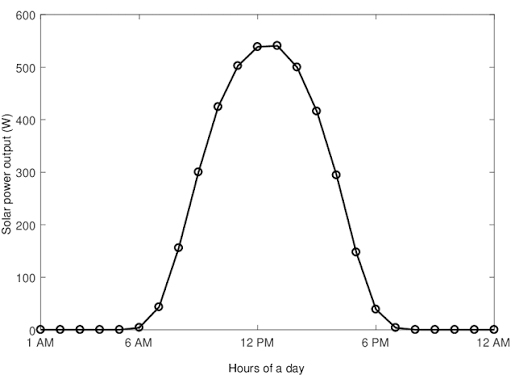
\includegraphics[width=\linewidth]{solar_generation photo.png}
\vspace{0.2cm}
\small Solar generation (Jahid, 2018).

\end{columns}
\end{frame}

\begin{frame}
\frametitle{Past studies}
\begin{itemize}
    \item Sun et al. reviewed over 500,000 US households and found that 60\% of them  could reduce electricity costs by an average of 15\% 
     \begin{itemize}
                \item 63\% of them could achieve affordable back-up power during power outages that could cover an average of 51\% of their essential energy needs 
    \end{itemize}
    \item Tervo et al. found that the long-term economic value of PV-battery systems depends on the state's electricity prices and incentives with high export prices
\end{itemize}
\end{frame}

\begin{frame}
\frametitle{Goal}
Investigate the economic feasibility of residential PV-battery storage systems for homeowners by identifying the battery capacity that minimizes electricity purchase costs while balancing the tradeoff between operational savings and battery ownership costs during summer and winter months. 
\end{frame}

\begin{frame}
\frametitle{San Diego location}
\begin{columns}[c]
    \column{0.4\textwidth}
    \centering
    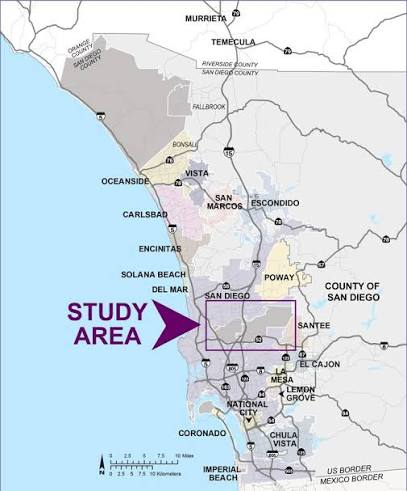
\includegraphics[width=\linewidth]{sandiegomap.jpeg}
    \column{0.4\textwidth}
    \begin{itemize}
        \item High electricity prices and high solar potential
        \item Weekday prices higher than weekend
    \end{itemize}
\end{columns}
\end{frame}
    
\begin{frame}
\frametitle{Data collection}
\begin{itemize}
    \item Open Energy Data Initiative's residential hourly load profiles
    \item National Renewable Energy Laboratory's (NREL) PVWatts® Version 8 calculator for solar generation profiles
    \item SDG\&E time-of-use electricity tariffs and Net Billing Tariff (NBT) export prices 
\end{itemize}
\end{frame}

\begin{frame}
\frametitle{Residential load profiles}
\begin{itemize}
    \item Generated using Energy Plus, a building simulation that represents a single-family detached home
    \item Simulated using Typical Meteorological Year 3 (TMY3) weather data
    \item BASE case for San Diego Miramar location
\end{itemize}
\end{frame}

\begin{frame}
\frametitle{Fourier Transform}
\vspace{-1cm}
\begin{block}{What is the Fourier Transform?}
The Fourier Transform is a mathematical technique that decomposes a signal into a combination of sinusoidal waves (sines and cosines) of different frequencies.
\end{block}
\begin{block}{Application}
Fast Fourier Transform (FFT) was used to identify and preserve the dominant repeating patterns in the residential load data while filtering out random fluctuations.
\end{block}
\end{frame}
    
\begin{frame}
\frametitle{FFT vs. Averaging}
\begin{columns}[c]
    \column{0.5\textwidth}
    \centering
    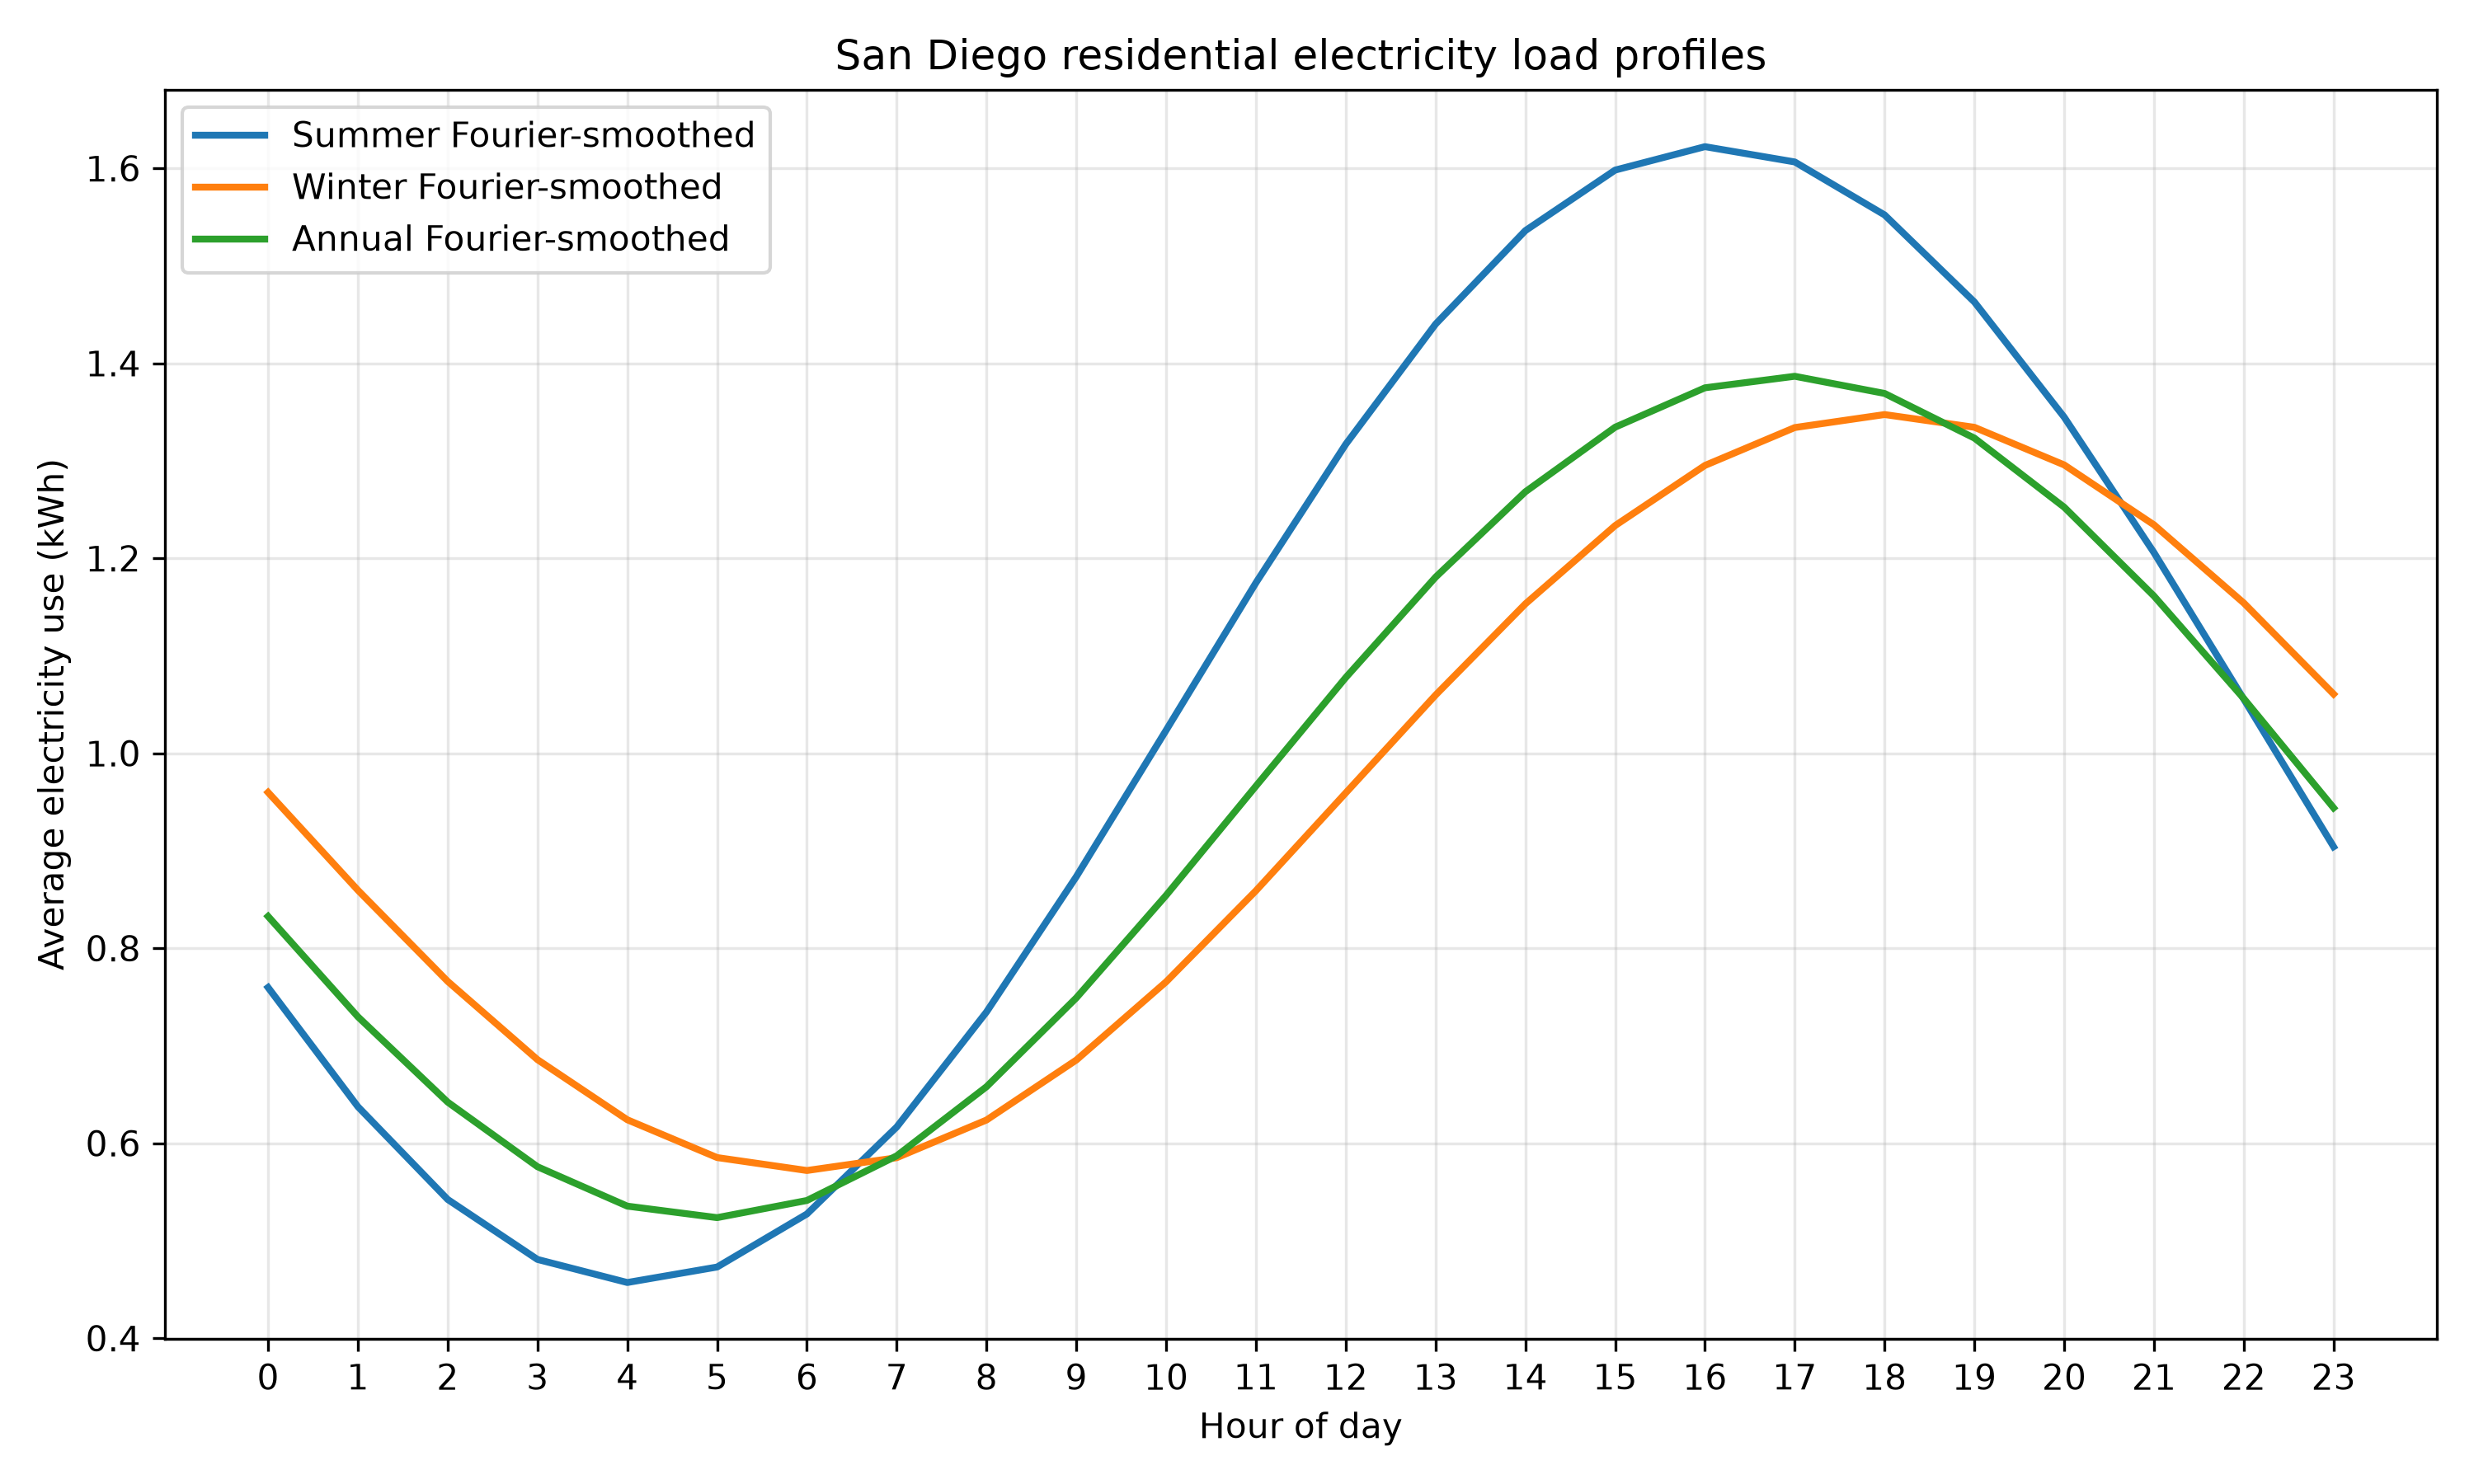
\includegraphics[width=\linewidth]{san_diego_load_profiles_fourier.png}
    \column{0.5\textwidth}
    \centering
    
\includegraphics[width=\linewidth]{san_diego_load_profiles.png}
\end{columns}
\end{frame}

\begin{frame}
\frametitle{Solar generation profiles}
\begin{itemize}
    \item National Renewable Energy Laboratory's (NREL) PVWatts® Version 8 calculator
    \item  PVWatts estimates the hourly electricity generation of a PV system based on system characteristics, geographic location, and historical weather data.
    \item Coordinates for San Diego Miramar location
\end{itemize}
\end{frame}

\begin{frame}
\frametitle{Seasonal solar profiles}
\begin{columns}[c]
    \column{0.6\textwidth}
    \centering
    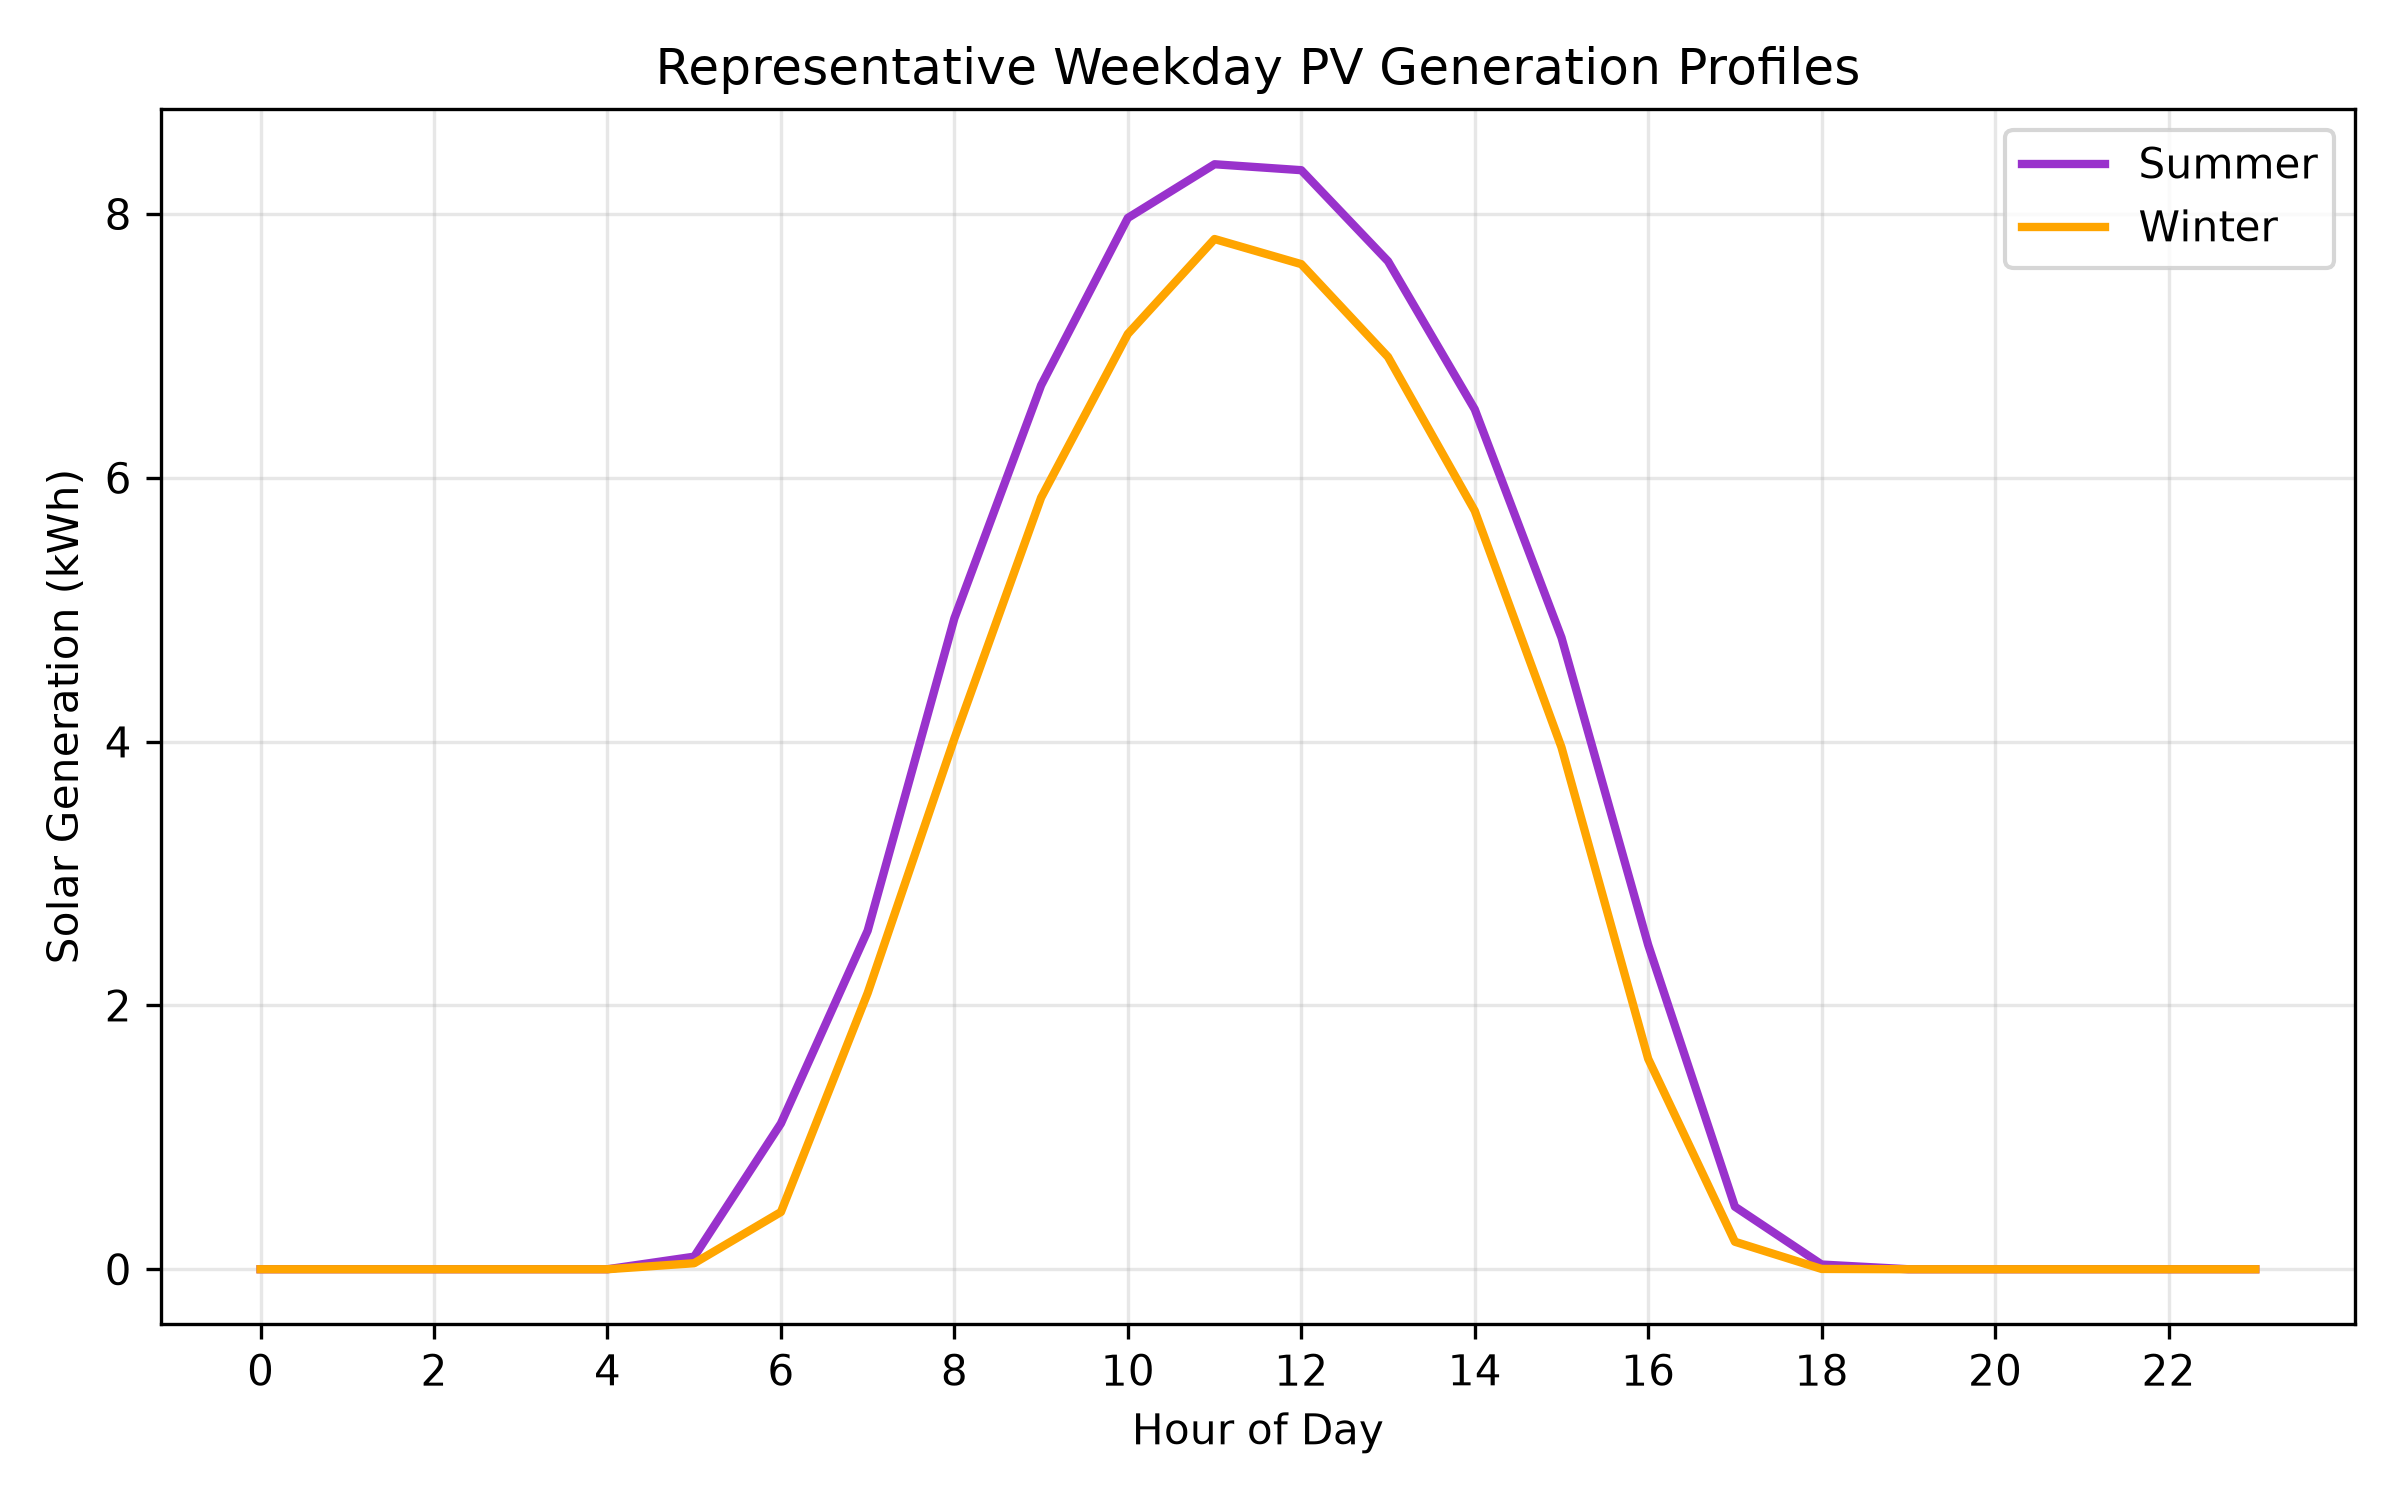
\includegraphics[width=\linewidth]{seasonal_solar_profiles.png}
    \column{0.4\textwidth}
    \begin{itemize}
        \item Size of PV system was 6 kW
        \item Tilt of the solar panels was 25° and the azimuth angle was set to 180° due to San Diego's latitude
        \item All set to the PVWatts default assumption values. 
    \end{itemize}
\end{columns}
\end{frame}

\begin{frame}
\frametitle{TOU pricing}
\begin{columns}[T]
    \column{0.45\textwidth}
    \centering
    \begin{tabular}{|c|r|}
    \hline
    \textbf{Period} & \textbf{Rate (\$/kWh)} \\
    \hline
    1 & 0.71598 \\
    2 & 0.38853 \\
    3 & 0.34545 \\
    4 & 0.50219 \\
    5 & 0.37682 \\
    6 & 0.33764 \\
    \hline
    \end{tabular}

    \column{0.55\textwidth}
    \centering
    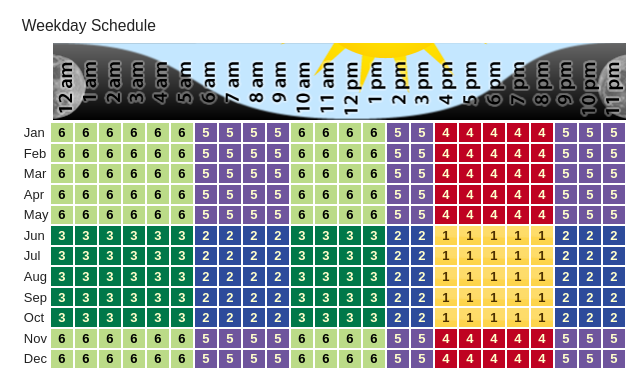
\includegraphics[width=\linewidth]{tou_pricing.png}
\end{columns}
\end{frame}

\begin{frame}
\frametitle{Export credits}

\begin{columns}[T]
    \column{0.45\textwidth}
    \begin{itemize}
        \item NEM 3.0 ended net metering
        \item Energy Export Credit is calculated as the sum of the corresponding Generation and Delivery components
        \item Rates locked-in for next nine years
    \end{itemize}

    \column{0.6\textwidth}
    \centering
    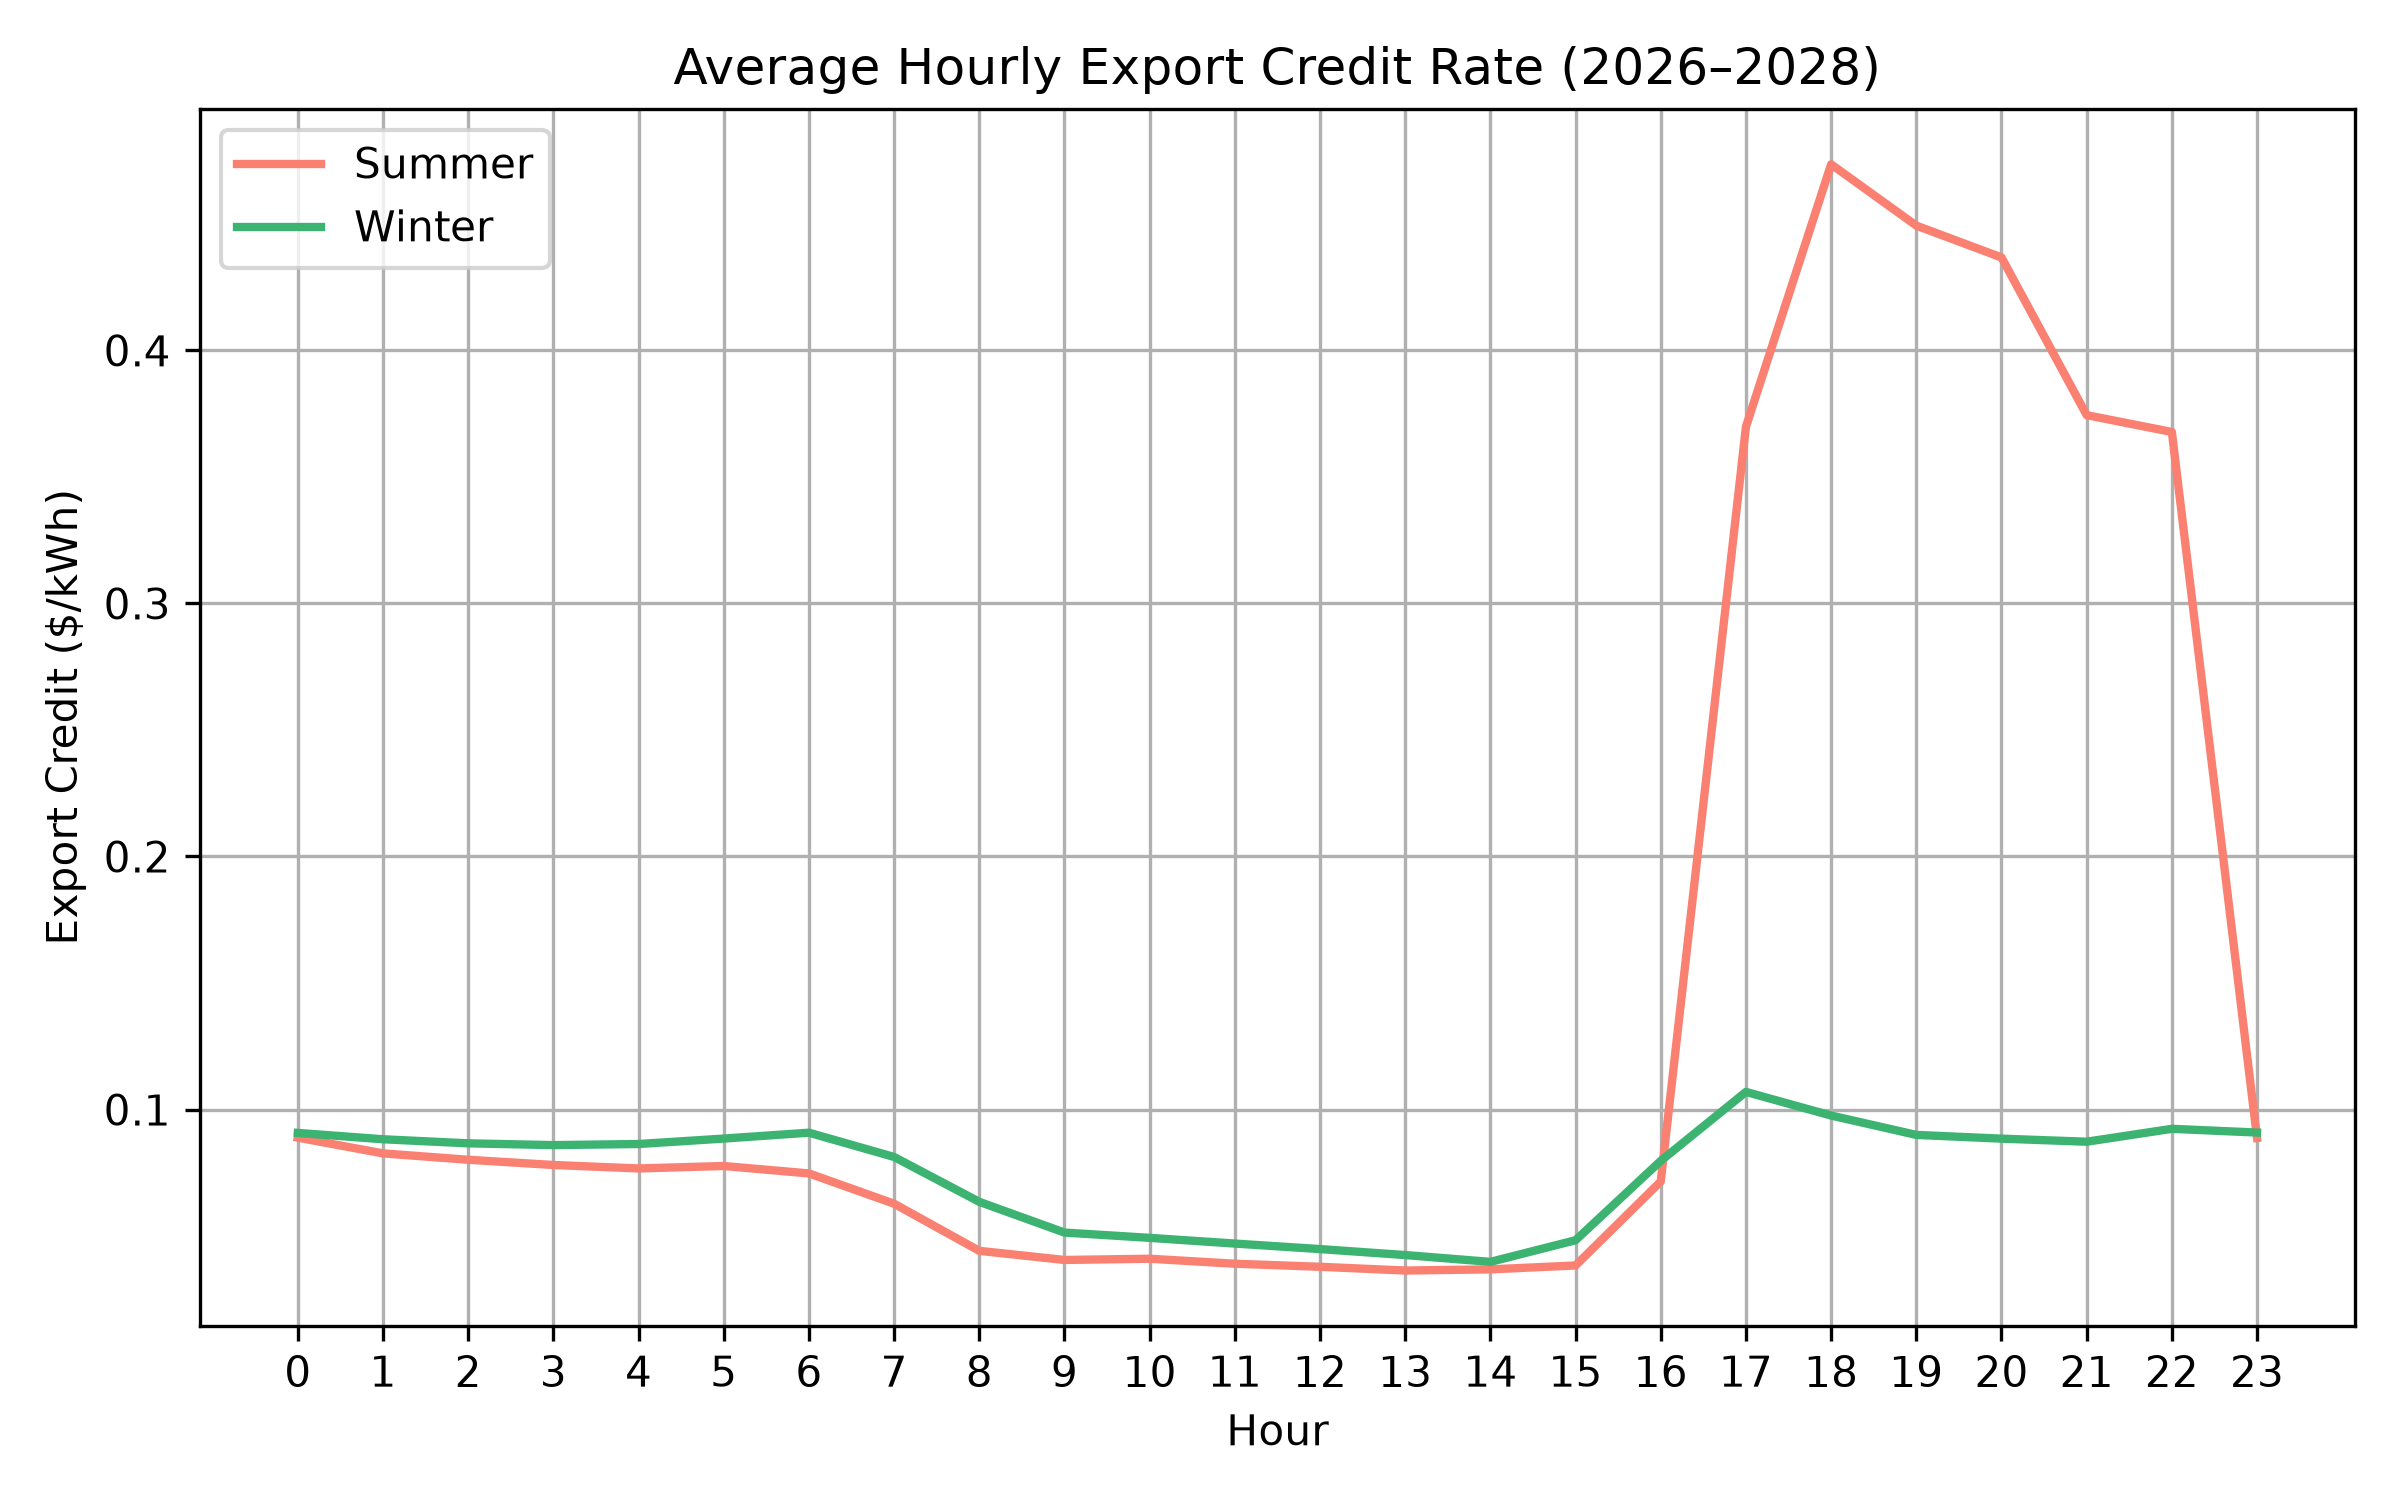
\includegraphics[width=\linewidth]{export_profile_2026_2028.png}
\end{columns}
\end{frame}

\begin{frame}
\frametitle{Cost minimization model}
\begin{itemize}
    \item Battery capacity that minimizes the cost of electricity for a residential PV-battery system by optimizing battery dispatch across multiple battery sizes. 
    \item Optimization variables include battery state of charge, grid electricity imports, grid electricity exports, battery charging from PV, and battery discharging to meet household electricity demand.
\end{itemize}
\end{frame}

\begin{frame}
\frametitle{Amortized capital cost}
\vspace{-1cm}
\begin{block}{Capitalized Recovery Factor}
Converts the battery's upfront capital cost into an equivalent annual cost over its expected lifetime while accounting for the time value of money
\end{block}

\begin{equation}
\mathrm{CRF} =
\frac{r(1+r)^n}{(1+r)^n-1},
\end{equation}

\begin{equation}
C_{\mathrm{annual}}
=
C_{\mathrm{net}}
\times
\mathrm{CRF},
\end{equation}
\end{frame}

\begin{frame}
\frametitle{Overall results}
\begin{table}[H]
\centering
\begin{tabular}{lcc}
\toprule
\textbf{Metric} & \textbf{Summer} & \textbf{Winter} \\
\midrule
Optimal Battery Capacity (kWh) & 12 & 10 \\
Daily Operating Cost (\$) & -0.24 & 0.35 \\
Daily Bill Savings (\$) & 4.76 & 3.29 \\
Annualized Capital Cost (\$/yr) & 1025.12 & 854.27 \\
Daily Net Benefit (\$) & 1.95 & 0.95 \\
Annual Net Benefit (\$/yr) & 711.75 & 346.75 \\
\bottomrule
\end{tabular}
\end{table}
\end{frame}

\begin{frame}
\frametitle{Net benefit vs. size curve}
\begin{columns}[c]
    \column{0.5\textwidth}
    \centering
    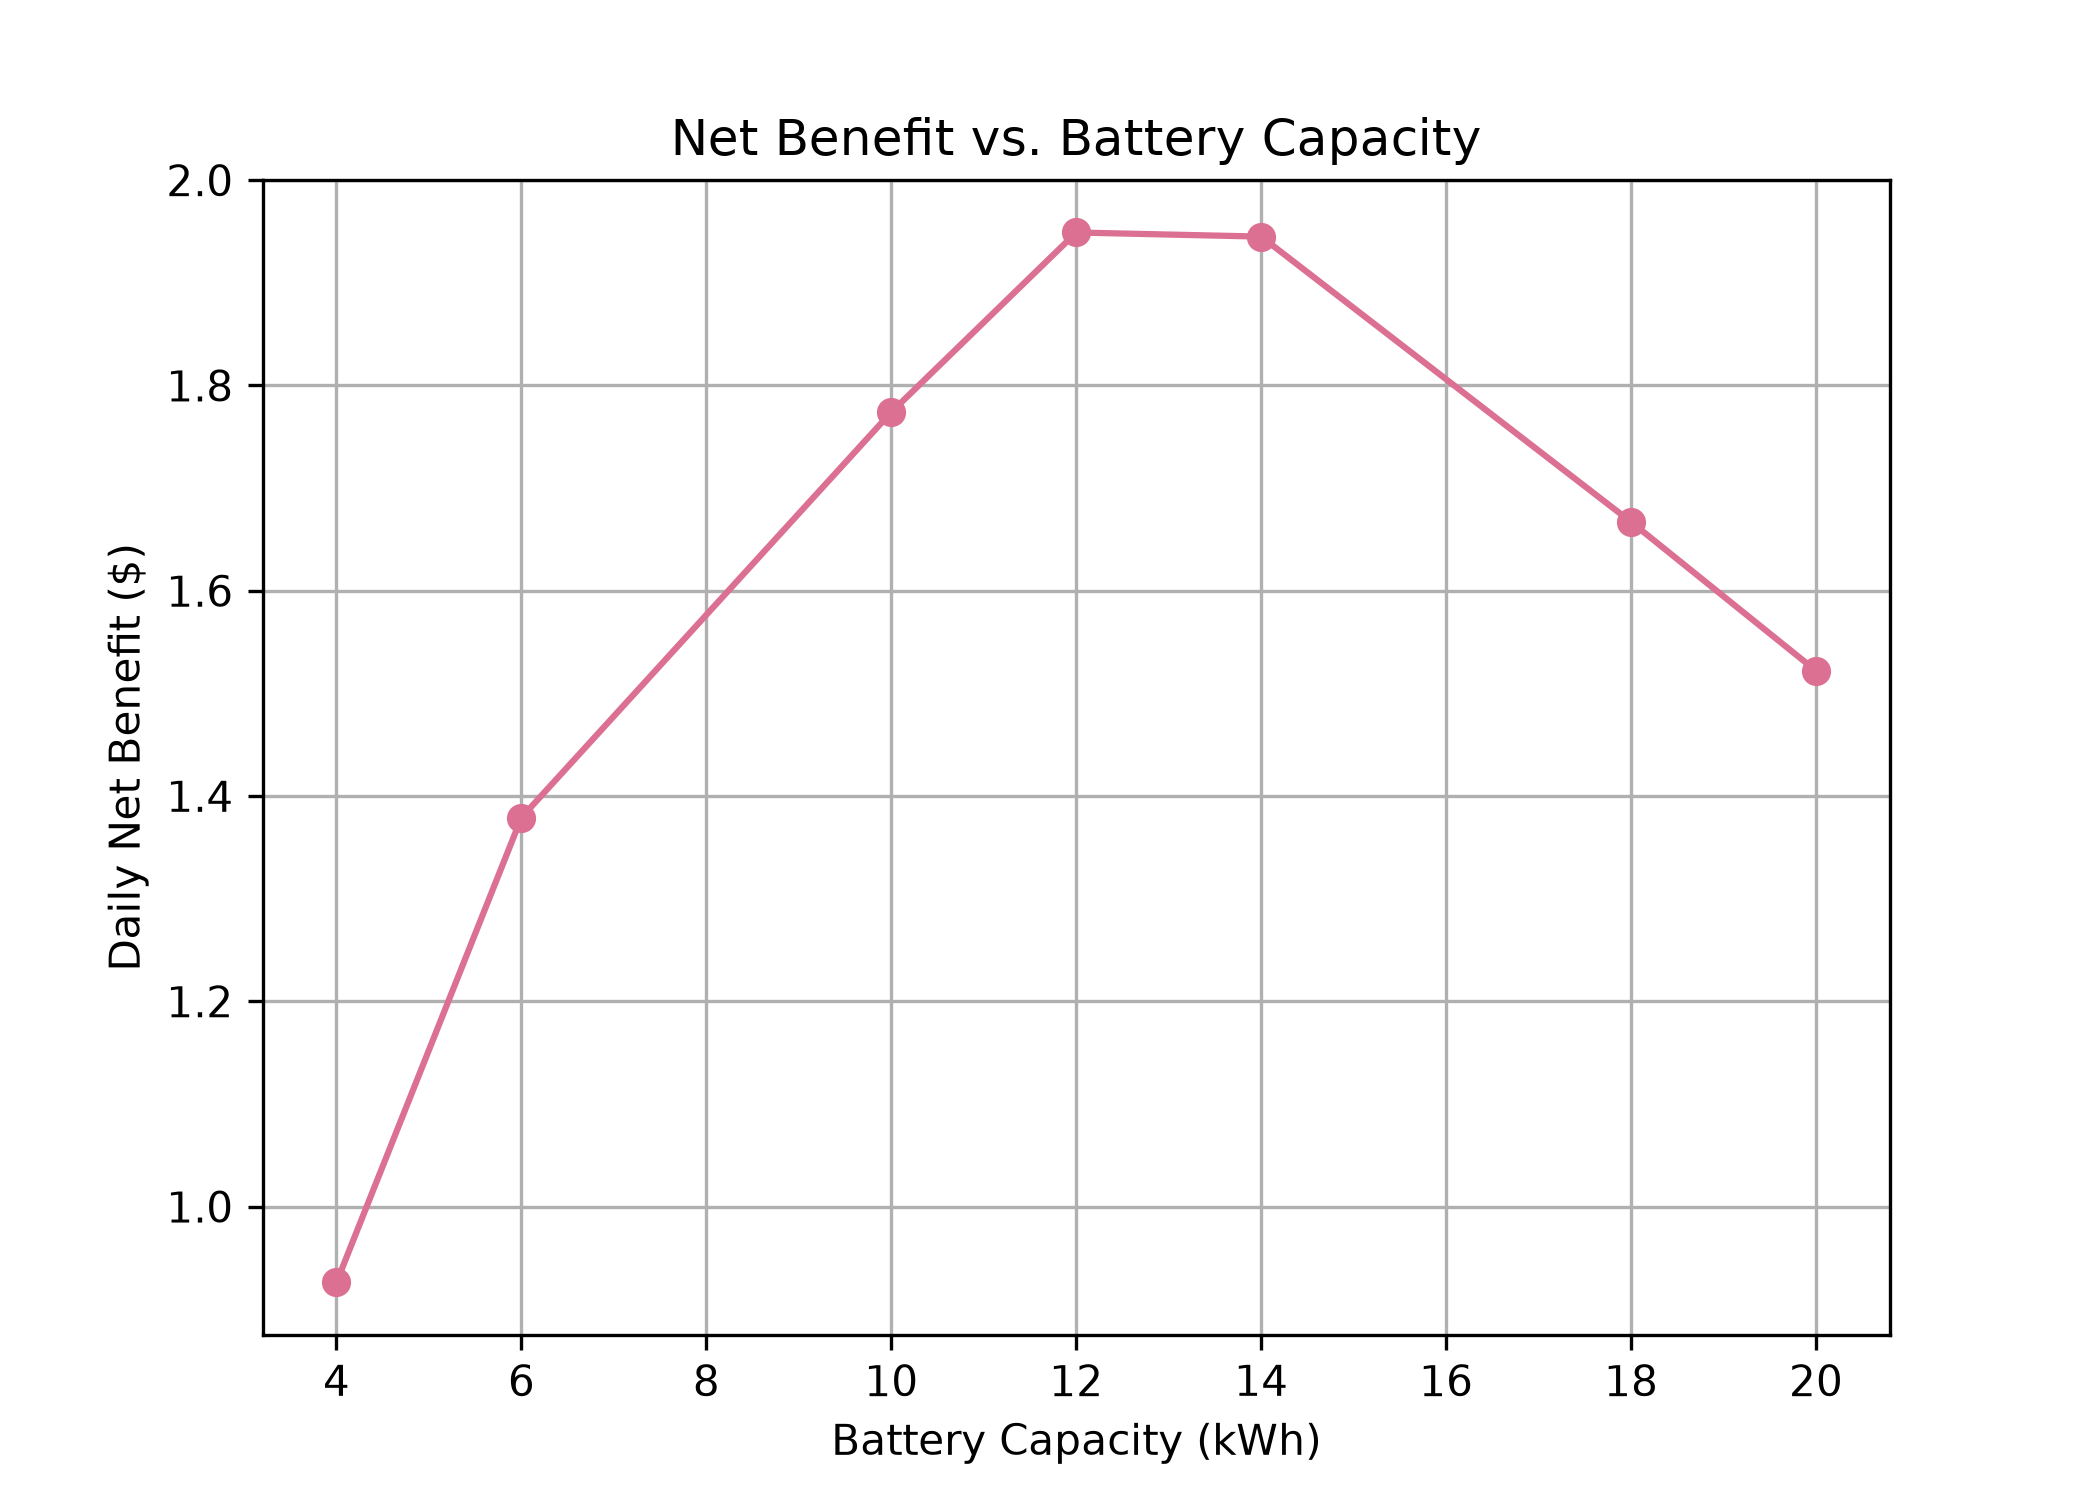
\includegraphics[width=\linewidth]{summer_net_benefit_vs_capacity.png}
    \vspace{0.2cm} 
    \small Summer
    \column{0.5\textwidth}
    \centering
    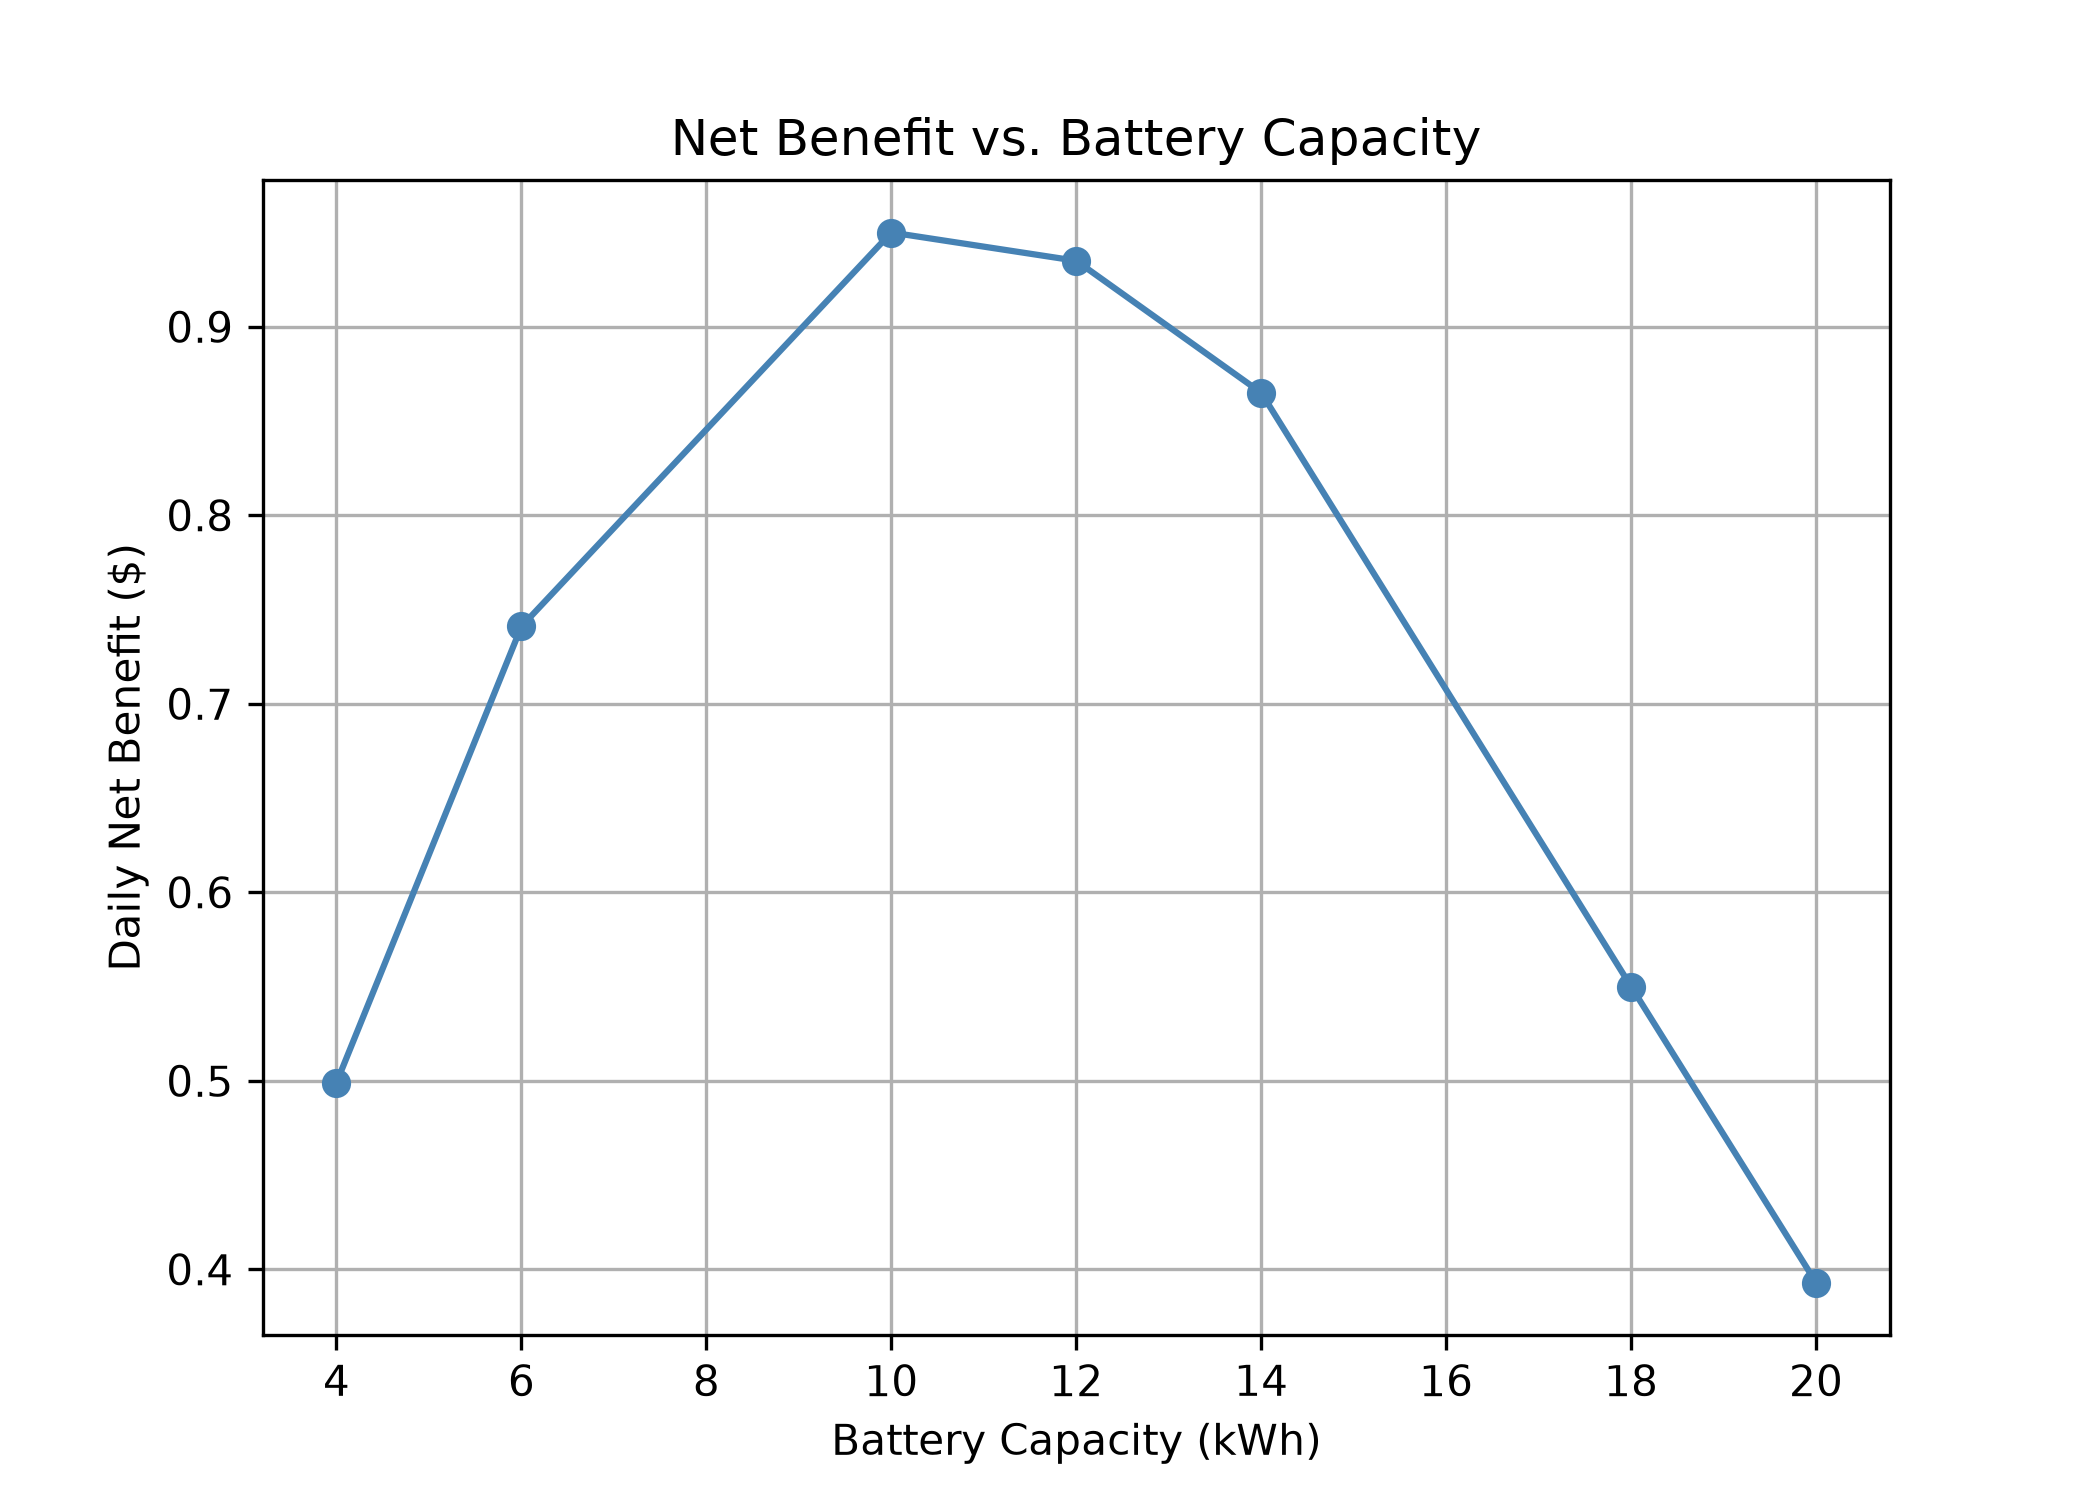
\includegraphics[width=\linewidth]{winter_net_benefit_vs_capacity.png}
    \vspace{0.2cm}
    \small Winter
 
\end{columns}
\end{frame}

\begin{frame}
\frametitle{Analysis of results}
\begin{itemize}
    \item The optimal battery capacity is larger in summer (12 kWh) than in winter (10 kWh) due to greater solar generation 
    \item Intermediate battery size does better
    \item  Seasonal solar generation and TOU pricing strongly influenced affordability
\end{itemize}
\end{frame}

\begin{frame}
\frametitle{Limitations and future research}
{\Large
\begin{itemize}
    \item Only one location; future work could expand the analysis to other regions.
    \item Operation and maintenance costs
    \item Day-to-day variability.
\end{itemize}
}
\end{frame}

\begin{frame}
\frametitle{Thank You!}
\centering
\LARGE Questions?
\end{frame}

\end{document}
